\documentclass{article}
\linespread{1.3}
\usepackage[margin=50pt]{geometry}
\usepackage{amsmath, amsthm, amssymb, amsthm,fancyhdr, graphicx, tikz}
\pagestyle{fancy}
\renewcommand{\headrulewidth}{0pt}
\newcommand{\changefont}{\fontsize{15}{15}\selectfont}

\fancypagestyle{firstpageheader}
{
  \fancyhead[R]{\changefont Michael Huang \\ Homework 6 \\ Adekoya}
}

\begin{document}

\thispagestyle{firstpageheader}

\section*{2.}
{\Large
The random variable $X$ has the following probability density function:
\[
f\left(t\right)=\begin{cases}
ct^{2} & \,-1\le t\le,2;\\
0 & \,\mbox{otherwise,}
\end{cases}
\]
where $c$ is a constant.

\subsection*{(a)}
To find $c$, we aim to solve for $c$ in the equation $\int_{-1}^{2}  ct^2\,dx = 1$, since we know that the total probability must be 1. Solving this: \\ 
$\frac{ct^3}{3}|_{-1}^{2} = 1$ \\ 
$\frac{8c}{3} + \frac{c}{3} = 1$ \\ 
$3c = 1$
$c = \frac{1}{3}$

\begin{figure}[ht!]
  \centering
  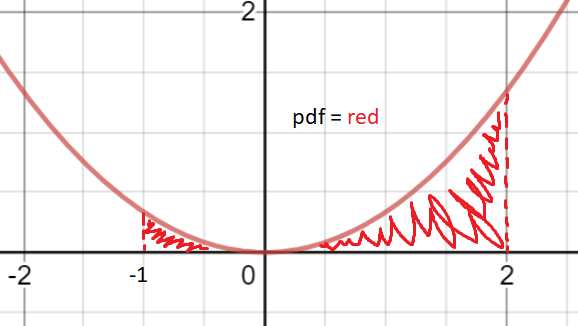
\includegraphics[width=90mm]{pdf.PNG}
  \caption{A simple caption \label{overflow}}
\end{figure}

\subsection*{(b)}


\subsection*{(c)}


\subsection*{(d)}


}

\section*{3.}
{\Large 

\subsection*{(a)}


\subsection*{(b)}


\subsection*{(c)}


\subsection*{(d)}


}

\section*{4.}
{\Large 



}

\section*{5.}
{\Large 



}

\section*{6.}
{\Large 



}

\section*{7.}
{\Large 



}

\section*{8.}
{\Large 



}

\section*{9.}
{\Large 

\subsection*{(a)}


\subsection*{(b)}


\subsection*{(c)}


\subsection*{(d)}


}

\end{document}